\chapter{Escores e confiabilidade de questionários}
\label{cap:confiabilidade}

Muitas pesquisas usam várias perguntas para descrever um tema, como hábitos de estudo, percepção de uma atividade ou satisfação com um serviço. Antes de comparar médias ou ajustar uma regressão, precisamos entender como as respostas se tornam um escore e quais interpretações ele sustenta.

Neste capítulo, vamos organizar cinco itens, recodificar um item invertido, construir um total e examinar a consistência interna. Usaremos um questionário \textbf{inteiramente fictício}, com 30 respostas construídas para ensino. Ele não é um instrumento validado e não deve ser apresentado como uma escala pronta para aplicação em pesquisas.

\section{Do conceito às perguntas}

Um conceito como ``hábitos de estudo'' não corresponde a uma coluna observada diretamente. Precisamos definir o que pretendemos representar, formular perguntas compreensíveis e estabelecer como cada resposta participa da pontuação. A qualidade dessa definição vem antes do cálculo de um coeficiente.

No arquivo \texttt{exemplo\_escalas.csv}, os itens ilustrativos são:

\begin{enumerate}
  \item Reservo um horário para estudar.
  \item Organizo as atividades que preciso realizar.
  \item Deixo de realizar as atividades de estudo que planejei.
  \item Reviso o conteúdo depois das aulas.
  \item Acompanho meu progresso nas atividades de estudo.
\end{enumerate}

Cada resposta vai de 1, Discordo totalmente, a 5, Concordo totalmente. Os itens 1, 2, 4 e 5 foram escritos em direção favorável aos hábitos propostos. O terceiro foi escrito na direção oposta. Os enunciados foram criados apenas para tornar a recodificação concreta; não houve estudo de conteúdo, compreensão ou estrutura desse questionário.

Os \textit{Standards for Educational and Psychological Testing}, de AERA, APA e NCME, distinguem a precisão dos escores e as evidências que sustentam sua interpretação para um uso. Um coeficiente de consistência interna não substitui esse conjunto de evidências \parencite{Standards2014}.

\section{Conferindo as respostas e a direção dos itens}

Abra o CSV no jamovi. Cada linha representa uma pessoa, e as cinco colunas de itens contêm suas respostas. Use \texttt{id} como identificador. Os itens têm dados inteiros e medida ordinal, com a ordem 1, 2, 3, 4, 5. Faça primeiro tabelas de frequência e confira se há códigos fora desses limites, categorias vazias ou ausentes.

Uma categoria com código 9 para ``não respondeu'' não deve entrar na soma como se representasse concordância maior que 5. Defina os ausentes antes de calcular escores. Também não substitua automaticamente um ausente por zero: zero não pertence à escala de respostas deste exemplo.

\subsection{Recodificando o item invertido}

Para uma escala de respostas que vai do limite inferior $L$ ao superior $U$, a inversão é:
\[
X_{\mathrm{invertido}}=L+U-X.
\]
Com $L=1$ e $U=5$, temos $X_{\mathrm{invertido}}=6-X$. Uma resposta 1 passa a 5; 2 passa a 4; 3 permanece 3. O objetivo é alinhar a direção substantiva dos itens, e não fazer os resultados parecerem melhores.

\begin{figure}[H]
\centering
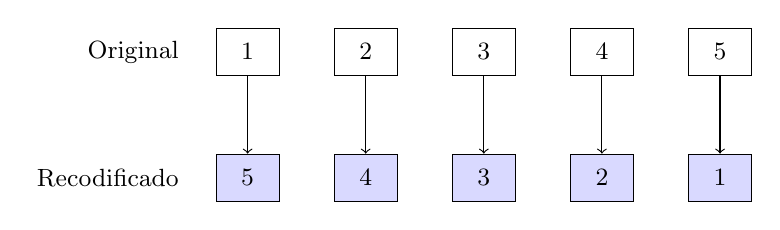
\begin{tikzpicture}[x=1.5cm,y=1cm,every node/.style={font=\small}]
  \node[left] at (-0.5,1.6) {Original};
  \node[left] at (-0.5,0) {Recodificado};
  \foreach \x/\a/\b in {0/1/5,1/2/4,2/3/3,3/4/2,4/5/1} {
    \node[draw,minimum width=0.8cm,minimum height=0.6cm] (a\x) at (\x,1.6) {\a};
    \node[draw,fill=blue!15,minimum width=0.8cm,minimum height=0.6cm] (b\x) at (\x,0) {\b};
    \draw[->] (a\x) -- (b\x);
  }
\end{tikzpicture}
\caption{Correspondência da inversão $6-X$ para respostas de 1 a 5. A posição de cada coluna indica a correspondência, não uma nova ordenação dos participantes. Elaboração própria.}
\label{fig:inversao-item}
\end{figure}

Crie uma variável calculada \texttt{item3\_corr} com a expressão \texttt{6 - item3\_neg}. Preserve a coluna original e confira a correspondência nas frequências. No primeiro registro do arquivo, \texttt{item3\_neg} vale 2; o valor corrigido deve ser 4. O capítulo de manipulação apresenta o uso de variáveis calculadas e a lista oficial de funções \parencite{JamoviFuncoes}.

Use os limites \textbf{teóricos} da escala de respostas. Se, em outro banco, ninguém marcou 1 ou 5, isso não muda a regra planejada de uma escala de 1 a 5. O painel de confiabilidade também oferece indicação de itens invertidos \parencite{JamoviConfiabilidade}; neste capítulo, usaremos a coluna já corrigida e não a inverteremos novamente no painel.

\section{Construindo um escore}

Depois de alinhar as direções, um total simples soma os cinco itens:
\[
T_i=X_{i1}+X_{i2}+X_{i3,\mathrm{corr}}+X_{i4}+X_{i5}.
\]
Se todos variam de 1 a 5 e estão completos, o total varia de 5 a 25. Uma média de itens usa:
\[
M_i=\frac{T_i}{5},
\]
com valores entre 1 e 5. No primeiro registro, os itens corrigidos são $4,4,4,3,4$: o total é 19 e a média é 3,8.

No jamovi, crie \texttt{total\_estudo} com \texttt{item1 + item2 + item3\_corr + item4 + item5}. Depois crie \texttt{media\_estudo} com \texttt{total\_estudo / 5}. Confira manualmente uma linha antes de usar o escore em outra análise.

A soma e a média são transformações lineares do mesmo escore quando todas as pessoas respondem aos mesmos cinco itens com os mesmos pesos. A posição relativa das pessoas não muda; as unidades e os limites mudam. No arquivo, a média dos totais é aproximadamente $14{,}767$, com DP $6{,}229$. A média dos escores médios é $2{,}953$, com DP aproximadamente $1{,}246$.

Somar respostas ordinais pressupõe uma regra de pontuação que precisa ser justificada para o uso. O ato de calcular a média não demonstra que as distâncias subjetivas entre Discordo totalmente e Discordo sejam idênticas às de outras categorias. Para um instrumento existente, siga seu manual e as evidências disponíveis, inclusive regras de pontuação e tratamento de ausentes.

\subsection{Quando faltam respostas}

É diferente exigir cinco respostas, aceitar quatro de cinco ou substituir itens ausentes por uma média. Essas escolhas podem alterar quem recebe escore e o que escores iguais significam. Defina a regra antes de olhar os resultados e informe quantas pessoas atenderam ao critério.

Nosso banco não contém ausentes, portanto todas as 30 pessoas possuem os cinco itens. Para uma atividade, faça uma cópia e apague uma resposta. Observe o que ocorre com a soma escrita com o operador \texttt{+} e com a análise de confiabilidade. Não suponha que o cálculo de um escore e a seleção de casos de outra análise usem automaticamente a mesma regra.

Uma média disponível calculada sobre apenas um item pode acabar colocada na mesma coluna que médias de cinco itens. Ter a mesma faixa numérica não torna a quantidade de informação igual. Quando o manual autorizar pontuação parcial, registre também a quantidade de itens respondidos.

\section{Covariância: por que os itens se relacionam?}

A consistência interna depende das relações entre itens. Para dois itens numéricos, a covariância amostral é:
\[
s_{jk}=\frac{1}{n-1}\sum_{i=1}^{n}
(X_{ij}-\bar{X}_j)(X_{ik}-\bar{X}_k).
\]
Quando pessoas acima da média de um item tendem também a ficar acima da média do outro, a covariância tende a ser positiva. A correlação divide a covariância pelo produto dos desvios padrão, retirando as unidades:
\[
r_{jk}=\frac{s_{jk}}{s_js_k}.
\]
Um item invertido ainda não recodificado pode apresentar covariâncias negativas com os demais. Isso pode ser um problema de direção da pontuação, sem significar que o conteúdo deva ser eliminado.

A variância do total depende das variâncias dos itens e de suas covariâncias:
\[
s_T^2=\sum_{j=1}^{k}s_j^2+2\sum_{j<l}s_{jl}.
\]
A soma dos cinco itens, portanto, não tem variância igual apenas à soma das cinco variâncias. Os produtos cruzados importam. A figura~\ref{fig:matriz-itens} mostra as correlações do banco após a correção do terceiro item.

\begin{figure}[H]
\centering
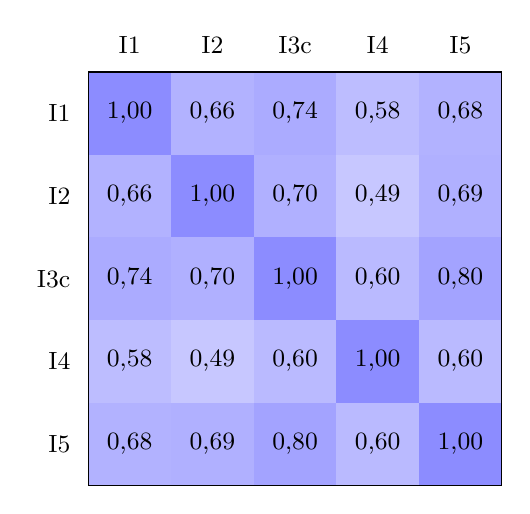
\begin{tikzpicture}[x=1.05cm,y=1.05cm,every node/.style={font=\small}]
  \fill[blue!45] (0,4) rectangle ++(1,1);
  \node at (0.5,4.5) {1,00};
  \fill[blue!30] (1,4) rectangle ++(1,1);
  \node at (1.5,4.5) {0,66};
  \fill[blue!33] (2,4) rectangle ++(1,1);
  \node at (2.5,4.5) {0,74};
  \fill[blue!26] (3,4) rectangle ++(1,1);
  \node at (3.5,4.5) {0,58};
  \fill[blue!30] (4,4) rectangle ++(1,1);
  \node at (4.5,4.5) {0,68};
  \fill[blue!30] (0,3) rectangle ++(1,1);
  \node at (0.5,3.5) {0,66};
  \fill[blue!45] (1,3) rectangle ++(1,1);
  \node at (1.5,3.5) {1,00};
  \fill[blue!31] (2,3) rectangle ++(1,1);
  \node at (2.5,3.5) {0,70};
  \fill[blue!22] (3,3) rectangle ++(1,1);
  \node at (3.5,3.5) {0,49};
  \fill[blue!31] (4,3) rectangle ++(1,1);
  \node at (4.5,3.5) {0,69};
  \fill[blue!33] (0,2) rectangle ++(1,1);
  \node at (0.5,2.5) {0,74};
  \fill[blue!31] (1,2) rectangle ++(1,1);
  \node at (1.5,2.5) {0,70};
  \fill[blue!45] (2,2) rectangle ++(1,1);
  \node at (2.5,2.5) {1,00};
  \fill[blue!27] (3,2) rectangle ++(1,1);
  \node at (3.5,2.5) {0,60};
  \fill[blue!36] (4,2) rectangle ++(1,1);
  \node at (4.5,2.5) {0,80};
  \fill[blue!26] (0,1) rectangle ++(1,1);
  \node at (0.5,1.5) {0,58};
  \fill[blue!22] (1,1) rectangle ++(1,1);
  \node at (1.5,1.5) {0,49};
  \fill[blue!27] (2,1) rectangle ++(1,1);
  \node at (2.5,1.5) {0,60};
  \fill[blue!45] (3,1) rectangle ++(1,1);
  \node at (3.5,1.5) {1,00};
  \fill[blue!27] (4,1) rectangle ++(1,1);
  \node at (4.5,1.5) {0,60};
  \fill[blue!30] (0,0) rectangle ++(1,1);
  \node at (0.5,0.5) {0,68};
  \fill[blue!31] (1,0) rectangle ++(1,1);
  \node at (1.5,0.5) {0,69};
  \fill[blue!36] (2,0) rectangle ++(1,1);
  \node at (2.5,0.5) {0,80};
  \fill[blue!27] (3,0) rectangle ++(1,1);
  \node at (3.5,0.5) {0,60};
  \fill[blue!45] (4,0) rectangle ++(1,1);
  \node at (4.5,0.5) {1,00};
  \foreach \x/\nome in {0.5/I1,1.5/I2,2.5/I3c,3.5/I4,4.5/I5} {
    \node[above] at (\x,5.1) {\nome};
  }
  \foreach \y/\nome in {4.5/I1,3.5/I2,2.5/I3c,1.5/I4,0.5/I5} {
    \node[left] at (-0.1,\y) {\nome};
  }
  \draw (0,0) rectangle (5,5);
\end{tikzpicture}
\caption{Correlações de Pearson entre os cinco itens nos dados fictícios; I3c é o item corrigido. A intensidade do azul acompanha a magnitude positiva. A diagonal vale 1 porque cada item está correlacionado consigo. Elaboração própria.}
\label{fig:matriz-itens}
\end{figure}

O mapa resume relações observadas. Ele não demonstra que exista apenas um fator nem que os itens cubram todo o conteúdo relevante do conceito. Aqui, usaremos covariâncias e correlações de Pearson sobre os códigos numéricos; análises baseadas em correlações policóricas para respostas ordinais envolvem outras suposições e procedimentos.

\section{Alfa de Cronbach, passo a passo}

Uma expressão para o alfa não padronizado, com $k$ itens, é:
\[
\alpha=\frac{k}{k-1}\left(1-\frac{\sum_{j=1}^{k}s_j^2}{s_T^2}\right).
\]
O coeficiente foi desenvolvido na discussão de estrutura interna de medidas \parencite{Cronbach1951}; a documentação do pacote \texttt{psych} apresenta sua forma baseada na matriz de variâncias e covariâncias \parencite{RevelleAlpha}.

Vamos fazer a conta com o nosso arquivo corrigido. Temos $k=5$, soma das variâncias dos itens de aproximadamente $10{,}737$ e variância do total de $38{,}806$:
\[
\alpha\approx\frac54\left(1-\frac{10{,}737}{38{,}806}\right)
\approx0{,}904.
\]
Se usássemos o terceiro item sem corrigir sua direção, encontraríamos aproximadamente $0{,}294$. Essa diferença ilustra a importância de compreender a pontuação antes de interpretar a estatística.

\subsection{Executando no jamovi}

\begin{enumerate}
  \item Abra \textbf{Análises $\rightarrow$ Fator $\rightarrow$ Análise de confiabilidade (Reliability Analysis)}.
  \item Mova \texttt{item1}, \texttt{item2}, \texttt{item3\_corr}, \texttt{item4} e \texttt{item5} para a lista de itens. Não inclua o identificador, o total ou a média junto aos itens.
  \item Solicite alfa de Cronbach, ômega de McDonald, médias e desvios padrão dos itens, correlação item--resto e alfa se o item for excluído.
  \item Solicite o mapa de correlações e confira se a direção dos itens está alinhada. Como já corrigimos o item 3, deixe vazia a lista de itens a inverter.
\end{enumerate}

As opções de alfa, ômega, estatísticas dos itens e correlações são documentadas pelo projeto jamovi \parencite{JamoviConfiabilidade}. Para conferir o alfa, espere aproximadamente $0{,}904$ com os cinco itens corrigidos e as 30 pessoas do arquivo. Os números apresentados neste capítulo foram calculados diretamente do CSV, sem reproduzir uma captura de saída do programa.

\subsection{O que o alfa não demonstra}

O valor $0{,}904$ não significa que 90,4\% das respostas estejam corretas. Também não comprova que o questionário mede um único conceito ou que possa ser usado para classificar pessoas. Sua interpretação como estimativa de confiabilidade depende do modelo de medida, incluindo relações entre itens e erros; ela não decorre apenas de o número estar próximo de 1.

Em um modelo clássico, podemos escrever um escore observado como $X=T+E$, com componente verdadeiro e erro de média zero não correlacionado com o componente verdadeiro. A confiabilidade corresponde à razão $\operatorname{Var}(T)/\operatorname{Var}(X)$ no domínio de repetições especificado. Diferentes fontes de erro, como ocasião e avaliador, pedem desenhos diferentes. A consistência entre itens em uma única aplicação não avalia, sozinha, estabilidade temporal ou concordância entre avaliadores.

Um ponto de corte universal, como 0,70 para qualquer situação, omite o uso pretendido e a precisão necessária. A descrição de confiabilidade deve acompanhar o grupo, as condições e a forma de pontuação, como orientam os Standards \parencite{Standards2014}. No exemplo, estamos praticando um cálculo sobre dados construídos; não estimando a qualidade de um instrumento real.

\section{Quantidade de itens e alfa padronizado}

Se calculamos o alfa a partir das correlações, usando itens padronizados, sua expressão é:
\[
\alpha_{\mathrm{pad}}=\frac{k\bar r}{1+(k-1)\bar r},
\]
em que $\bar r$ é a média das correlações entre pares distintos de itens. O alfa padronizado e o não padronizado podem diferir quando as variâncias dos itens diferem \parencite{RevelleAlpha}.

No nosso banco, $\bar r\approx0{,}652$, produzindo alfa padronizado de aproximadamente $0{,}904$, muito próximo do não padronizado neste caso. Essa proximidade é uma característica dos números do exemplo, e não uma identidade geral entre os procedimentos.

A fórmula também mostra a relação com o número de itens. Mantendo uma correlação média hipotética de $0{,}30$, quatro itens produzem $\alpha_{\mathrm{pad}}\approx0{,}632$ e oito produzem aproximadamente $0{,}774$. Um coeficiente maior pode resultar de uma escala mais longa sem que cada item tenha se tornado individualmente melhor.

\begin{figure}[H]
\centering
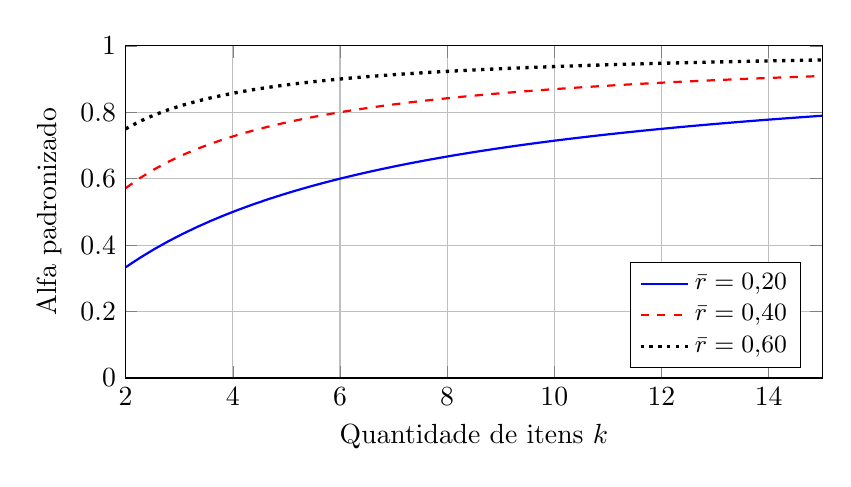
\begin{tikzpicture}
\begin{axis}[
  width=0.86\textwidth,height=5.8cm,
  xlabel={Quantidade de itens $k$},ylabel={Alfa padronizado},
  xmin=2,xmax=15,ymin=0,ymax=1,xtick={2,4,6,8,10,12,14},grid=major,
  legend style={at={(0.97,0.03)},anchor=south east,font=\small}
]
  \addplot[blue,thick,domain=2:15,samples=50] {x*0.2/(1+(x-1)*0.2)};
  \addlegendentry{$\bar r=0{,}20$}
  \addplot[red,dashed,thick,domain=2:15,samples=50] {x*0.4/(1+(x-1)*0.4)};
  \addlegendentry{$\bar r=0{,}40$}
  \addplot[black,dotted,very thick,domain=2:15,samples=50] {x*0.6/(1+(x-1)*0.6)};
  \addlegendentry{$\bar r=0{,}60$}
\end{axis}
\end{tikzpicture}
\caption{Relação algébrica entre quantidade de itens, correlação média e alfa padronizado. As linhas ligam valores da fórmula; uma quantidade fracionária de itens não é uma aplicação real. Elaboração própria.}
\label{fig:alpha-comprimento}
\end{figure}

Adicionar perguntas quase idênticas pode aumentar o coeficiente e, ao mesmo tempo, estreitar a cobertura do conceito ou tornar a aplicação cansativa. O planejamento deve considerar conteúdo, compreensão e utilidade, além da relação entre itens. A fórmula ajuda a interpretar uma mudança; não é uma instrução para maximizar o número a qualquer custo.

\section{Correlação item--resto e exclusão de itens}

A correlação item--resto relaciona um item com a soma dos \textbf{demais} itens:
\[
r_{j,\mathrm{resto}}=
\operatorname{cor}\left(X_j,\sum_{l\ne j}X_l\right).
\]
Excluir o próprio item da soma evita uma correlação parcialmente inflada pela presença da mesma resposta nos dois lados. A documentação do \texttt{psych} distingue essa estatística de correlações com o total completo \parencite{RevelleAlpha}.

\begin{table}[H]
\centering
\caption{Estatísticas por item nos dados corrigidos}
\begin{tabular}{lrr}
\hline
Item & Correlação item--resto & Alfa sem o item \\
\hline
1 & 0,774 & 0,881 \\
2 & 0,735 & 0,888 \\
3 corrigido & 0,843 & 0,864 \\
4 & 0,642 & 0,906 \\
5 & 0,815 & 0,871 \\
\hline
\end{tabular}
\label{tab:itens-confiabilidade}
\end{table}

Retirar o item 4 aumenta o alfa de aproximadamente $0{,}904$ para $0{,}906$, uma diferença pequena neste banco. Isso não basta para recomendar sua retirada. Precisamos perguntar qual conteúdo seria perdido, se o item foi compreendido e se o padrão se repete em dados adequados para avaliar o instrumento.

Uma correlação negativa pede conferir direção, codificação, erros de digitação e coerência do enunciado. Uma correlação muito alta também merece leitura de conteúdo, pois pode refletir redundância. Se houver revisão do instrumento, registre a justificativa e examine a nova versão em dados apropriados; selecionar itens e declarar sua qualidade no mesmo conjunto pode produzir uma avaliação otimista.

\section{Ômega e o modelo de medida}

O ômega de McDonald usa uma representação fatorial para distinguir variância comum e componentes específicos. A documentação do pacote \texttt{psych} apresenta versões do coeficiente e as escolhas de modelo envolvidas \parencite{RevelleOmega}. Não existe um único número chamado ômega que dispense identificar qual estrutura foi ajustada.

Para entender uma forma simples, considere um fator $F$ com variância 1, itens centrados e erros não correlacionados entre si e com o fator:
\[
X_j=\lambda_jF+\varepsilon_j,\qquad
\operatorname{Var}(\varepsilon_j)=\theta_j.
\]
A carga $\lambda_j$ liga o item ao fator. Sob esse modelo unifatorial, a proporção de variância comum no escore soma pode ser expressa por:
\[
\omega=\frac{\left(\sum_j\lambda_j\right)^2}
{\left(\sum_j\lambda_j\right)^2+\sum_j\theta_j}.
\]
Se permitirmos correlação entre erros, o denominador muda. Se a estrutura tiver vários fatores, precisamos distinguir, por exemplo, a contribuição total de fatores comuns e a de um fator geral. A fórmula acima não deve ser transportada automaticamente para qualquer estrutura.

\begin{figure}[H]
\centering
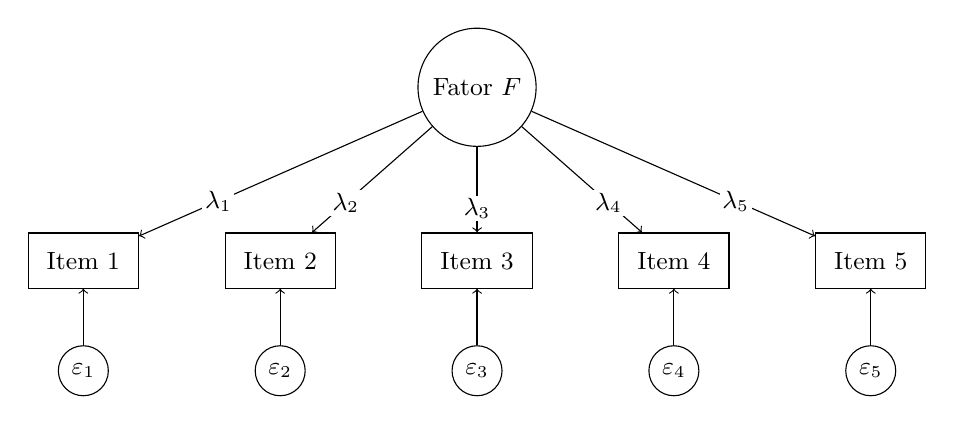
\begin{tikzpicture}[x=1cm,y=1cm,every node/.style={font=\small}]
  \node[draw,circle,minimum size=1.5cm] (fator) at (0,2.2) {Fator $F$};
  \foreach \x/\j in {-5/1,-2.5/2,0/3,2.5/4,5/5} {
    \node[draw,minimum width=1.4cm,minimum height=0.7cm] (i\j) at (\x,0) {Item \j};
    \node[draw,circle,inner sep=3pt] (e\j) at (\x,-1.4) {$\varepsilon_{\j}$};
    \draw[->] (fator) -- node[pos=0.72,fill=white,inner sep=1pt] {$\lambda_{\j}$} (i\j);
    \draw[->] (e\j) -- (i\j);
  }
\end{tikzpicture}
\caption{Modelo unifatorial hipotético para cinco itens alinhados. É um esquema de parâmetros, não o resultado de uma análise fatorial do nosso arquivo. Elaboração própria.}
\label{fig:modelo-medida}
\end{figure}

No jamovi, solicite ômega junto ao alfa para praticar a leitura, mas registre o procedimento e suas suposições. Um ômega alto também não prova o modelo nem substitui evidências sobre a interpretação do escore. Não apresentaremos um valor calculado de ômega como resultado esperado sem ajustar e avaliar o modelo correspondente.

\section{Erro de medida e precisão de um escore}
\label{sec:erro-medida-escore}

Voltemos ao modelo clássico $X=T+E$, com erros de média zero e não correlacionados com $T$. Se a confiabilidade no domínio de repetições definido for $\rho_{XX}=\operatorname{Var}(T)/\operatorname{Var}(X)$, então:
\[
\operatorname{Var}(E)=\operatorname{Var}(X)(1-\rho_{XX}),
\qquad \sigma_E=\sigma_X\sqrt{1-\rho_{XX}}.
\]
Essa relação permite representar um \textbf{erro padrão de medida} na unidade do escore. Em um modelo hipotético com DP observado 10 e confiabilidade $0{,}84$, temos $\sigma_E=10\sqrt{0{,}16}=4$ pontos. O número depende de qual fonte de erro e de quais repetições a confiabilidade representa; não basta substituir qualquer coeficiente disponível na fórmula.

\begin{figure}[H]
\centering
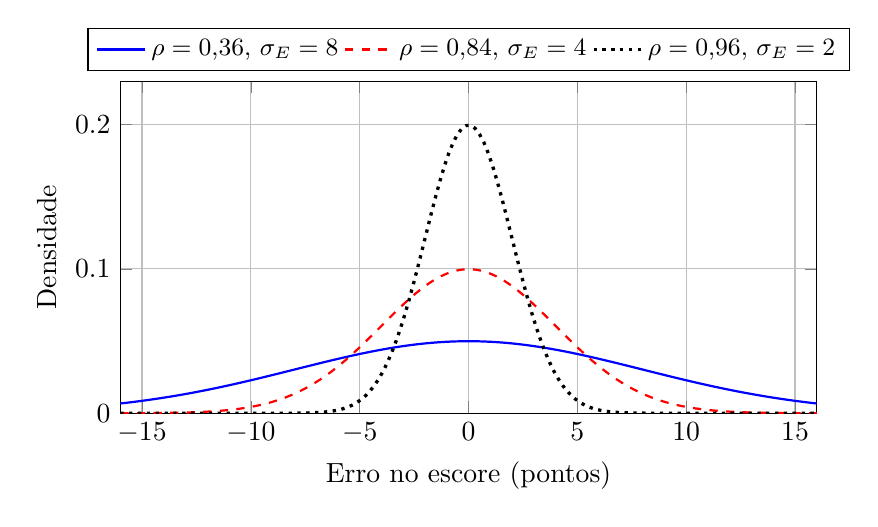
\begin{tikzpicture}
\begin{axis}[
  width=0.86\textwidth,height=5.8cm,
  xlabel={Erro no escore (pontos)},ylabel={Densidade},
  xmin=-16,xmax=16,ymin=0,ymax=0.23,grid=major,
  legend style={at={(0.5,1.03)},anchor=south,font=\small,legend columns=3}
]
  \addplot[blue,thick,domain=-16:16,samples=140]
    {exp(-(x/8)^2/2)/(8*sqrt(2*pi))};
  \addlegendentry{$\rho=0{,}36$, $\sigma_E=8$}
  \addplot[red,dashed,thick,domain=-16:16,samples=140]
    {exp(-(x/4)^2/2)/(4*sqrt(2*pi))};
  \addlegendentry{$\rho=0{,}84$, $\sigma_E=4$}
  \addplot[black,dotted,very thick,domain=-16:16,samples=160]
    {exp(-(x/2)^2/2)/(2*sqrt(2*pi))};
  \addlegendentry{$\rho=0{,}96$, $\sigma_E=2$}
\end{axis}
\end{tikzpicture}
\caption{Três modelos hipotéticos de erro normal, com DP observado fixado em 10. A curva se estreita quando a confiabilidade do modelo aumenta. A normalidade foi escolhida para o desenho e não é consequência da definição de confiabilidade. Elaboração própria.}
\label{fig:precisao-escore}
\end{figure}

Não confunda esse erro com o \textbf{erro padrão de uma média amostral}. A expressão $s_X/\sqrt n$, discutida no capítulo~\ref{cap:probabilidade}, trata da variabilidade da média entre amostras sob certas condições. O erro de medida se refere à precisão do escore no modelo de medição. Acrescentar participantes pode melhorar a estimação da média sem tornar as respostas de cada participante mais precisas.

A precisão também pode variar ao longo da escala; uma única medida global não descreve necessariamente todas as faixas de escore. Se uma aplicação envolve decisões individuais ou classificação por pontos de corte, consulte as evidências e o manual do instrumento para aquele uso. Os Standards relacionam a avaliação da precisão às interpretações e decisões pretendidas \parencite{Standards2014}. Nosso questionário fictício não fornece esse suporte.

\section{Consistência interna e estrutura são perguntas diferentes}

Um alfa ou ômega resume relações sob uma definição, mas a escolha de quais itens formam um escore exige examinar também seu conteúdo e sua estrutura. No modelo fatorial, itens são relacionados a variáveis latentes e a componentes específicos; na análise de componentes principais, construímos combinações das variáveis observadas para resumir sua variação. Os objetivos se aproximam em certas aplicações, mas os modelos não são idênticos.

No capítulo~\ref{cap:dimensoes}, vamos desenvolver essa distinção e os respectivos procedimentos no jamovi. Antes disso, retenha uma regra prática de leitura: um agrupamento estatístico de itens precisa de interpretação substantiva; receber um nome no gráfico não prova que um fator represente o conceito desejado.

Um total com pesos iguais e um escore derivado de coeficientes de um modelo também não são automaticamente a mesma medida. Documente como o escore foi calculado, em que dados o modelo foi estimado e se a regra é aplicável às pessoas que serão avaliadas. A possibilidade de calcular um número vem antes da questão principal: qual interpretação esse número sustenta?

\section{Como relatar e dar continuidade}

Um relato do exercício pode dizer: ``Nos 30 registros fictícios completos, foram examinados cinco itens de resposta de 1 a 5. O terceiro item foi recodificado por $6-X$ antes da pontuação. O alfa não padronizado foi $0{,}904$, e as correlações item--resto variaram de $0{,}642$ a $0{,}843$. Os valores ilustram o procedimento e não constituem evidência de validação do questionário.''

Em uma pesquisa, descreva os enunciados ou o instrumento original, o sistema de respostas, os itens invertidos, a regra de escore, os ausentes, a população e o método de estimação. A avaliação de estrutura fatorial, estabilidade temporal, concordância e relação com outras medidas depende da pergunta e de um desenho próprio. Nem toda fonte de erro é examinada com uma única aplicação de itens.

\begin{figure}[H]
\centering
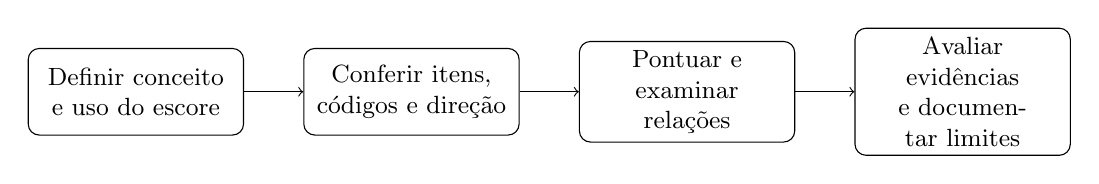
\begin{tikzpicture}[x=1cm,y=1cm,every node/.style={font=\small,align=center}]
  \node[draw,rounded corners,text width=2.5cm,minimum height=1.1cm] (a) at (0,0) {Definir conceito\\e uso do escore};
  \node[draw,rounded corners,text width=2.5cm,minimum height=1.1cm] (b) at (3.5,0) {Conferir itens,\\códigos e direção};
  \node[draw,rounded corners,text width=2.5cm,minimum height=1.1cm] (c) at (7,0) {Pontuar e\\examinar relações};
  \node[draw,rounded corners,text width=2.5cm,minimum height=1.1cm] (d) at (10.5,0) {Avaliar evidências\\e documentar limites};
  \draw[->] (a) -- (b);
  \draw[->] (b) -- (c);
  \draw[->] (c) -- (d);
\end{tikzpicture}
\caption{Etapas para construir e interpretar um escore. A definição de conteúdo orienta os cálculos e a documentação. Elaboração própria.}
\label{fig:roteiro-escore}
\end{figure}

\section{Vamos praticar: perguntas e comentários}

\begin{enumerate}
  \item Em uma resposta de 1 a 5, qual é o valor corrigido de um item invertido marcado como 2? E de um item marcado como 5?
  \item Para $4,4,4,3,4$, calcule total e média. Quais são os limites possíveis do total de cinco itens completos?
  \item Por que a variância do total não costuma ser apenas a soma das variâncias dos itens?
  \item O alfa de $0{,}904$ demonstra que o questionário é unidimensional e validado?
  \item O item 4 aumenta o alfa para $0{,}906$ quando excluído. Devemos removê-lo automaticamente?
  \item A consistência interna obtida em uma única aplicação demonstra estabilidade dos escores ao longo do tempo?
  \item Em um modelo com DP observado 10 e confiabilidade $0{,}84$, qual é o DP do erro de medida?
  \item Por que aumentar a amostra de 30 para 120 pessoas não garante que cada escore individual tenha menos erro de medida?
\end{enumerate}

\subsection*{Comentários das respostas}

\begin{enumerate}
  \item $6-2=4$ e $6-5=1$. A regra vem dos limites teóricos da escala.
  \item Total 19, média 3,8; os limites são 5 e 25. Essas relações pressupõem cinco itens completos com os mesmos pesos.
  \item Porque os termos de covariância também participam: $s_T^2=\sum s_j^2+2\sum_{j<l}s_{jl}$.
  \item Não. O coeficiente resume uma relação entre itens sob condições; estrutura e interpretação para um uso pedem outras evidências.
  \item Não. A diferença é pequena e precisa ser examinada com o conteúdo e a finalidade do item, além da incerteza e da possibilidade de confirmação em novos dados.
  \item Não. A estabilidade temporal requer um desenho com medidas em ocasiões adequadas; ela não se identifica somente pela relação entre itens na mesma aplicação.
  \item $10\sqrt{1-0{,}84}=4$ pontos, sob o modelo e o domínio de erro especificados.
  \item O tamanho amostral participa da precisão de estimativas populacionais. A precisão da medida individual depende do instrumento, das condições e do modelo de erro, que não melhoram automaticamente com mais pessoas.
\end{enumerate}

\section{Para continuar no Balaio Científico}

Para rever as operações que antecedem o cálculo de um escore, leia \href{https://www.balaiocientifico.com/2026/10/como-criar-uma-variavel-calculada-no.html}{Como criar uma variável calculada no Jamovi: soma e média} e \href{https://www.balaiocientifico.com/2026/10/valores-ausentes-no-jamovi-como-tratar.html}{Valores ausentes no Jamovi: como tratar códigos como 9999}.

Para localizar a ferramenta de cálculo de variáveis, acompanhe \href{https://www.youtube.com/watch?v=NBvQphd9FqI}{Jamovi - Calculadora Variáveis - Aula 9}.

\textbf{Vamos praticar:} Em \texttt{exemplo\_escalas.csv}, corrija o item invertido e calcule total e média. Confira o primeiro registro manualmente e descreva a regra para respostas ausentes antes de examinar a confiabilidade. O tutorial de cálculo apoia a operação; a interpretação dos coeficientes continua exigindo as condições discutidas neste capítulo.
